\section{گام اول: ساختاربندی پروژه و آماده‌سازی دادگان}

در این مرحله، هدف اصلی ایجاد بستر مناسب برای اجرای پروژه و پیاده‌سازی کلاس‌های مربوط به بارگذاری دادگان \lr{(Data Loading)} است. با توجه به نیازمندی‌های پروژه برای دسته‌بندی احساسات چهره، مجموعه داده‌ی \lr{FER2013} مورد استفاده قرار می‌گیرد.

\begin{stepbox}
\field{۱. پیکربندی و ساختار فایل‌ها}{
ساختار پروژه کاملاً ماژولار و بر اساس استانداردهای توسعه‌ی شبکه‌های عصبی عمیق طراحی شده است. کلیه‌ی هایپرپارامترهای کلیدی مانند نرخ یادگیری \lr{(learning rate)}، اندازه دسته \lr{(batch size)} و اندازه تصاویر \lr{(image size)} از داخل سورس‌کدها خارج شده و در فایل \texttt{config/config.yaml} متمرکز شده‌اند تا فرآیند تنظیم پارامترها \lr{(Tuning)} در مراحل بعدی بدون نیاز به تغییر کدها امکان‌پذیر باشد. ابعاد تصاویر ورودی برای هماهنگی با شبکه‌های از پیش آموزش‌دیده (مانند \lr{ResNet}) برابر با $224 \times 224$ تنظیم شده است.
}
\end{stepbox}

\subsection{پیش‌پردازش و افزونگی داده‌ها \lr{(Data Augmentation)}}

داده‌های \lr{FER2013} به‌صورت رشته‌هایی از پیکسل‌های تک‌کاناله \lr{(Grayscale)} ذخیره شده‌اند. برای امکان‌پذیر شدن استفاده از این تصاویر در معماری‌هایی که روی \lr{ImageNet} آموزش دیده‌اند، ابتدا رشته‌ها به آرایه‌های دوبعدی تبدیل شده و سپس با کپی کردن مقادیر، به تصاویر سه‌کاناله \lr{(RGB)} تعمیم یافتند.

\begin{tipbox}[جلوگیری از نشت اطلاعات \lr{(Data Leakage)}]
دقت شد که تکنیک‌های افزونگی داده \lr{(Augmentation)} منحصراً روی مجموعه‌ی آموزش \lr{(Training Split)} اعمال شوند و داده‌های اعتبارسنجی \lr{(PublicTest)} و آزمون \lr{(PrivateTest)} تنها فرآیندهای تغییر ابعاد و نرمال‌سازی را طی کنند.
\end{tipbox}

تغییرات اعمال شده روی مجموعه‌ی آموزش شامل موارد زیر است:
\begin{itemize}
    \item \textbf{چرخش تصادفی \lr{(Random Rotation)}:} چرخش ملایم تا حداکثر ۱۰ درجه برای شبیه‌سازی کجی سر.
    \item \textbf{انعکاس افقی \lr{(Horizontal Flip)}:} برای یادگیری ویژگی‌های تقارن چهره.
    \item \textbf{تغییرات روشنایی \lr{(Color Jitter)}:} تغییر ملایم روشنایی و کنتراست (تا ۲۰ درصد) برای مقاوم‌سازی مدل نسبت به شرایط نوری محیط.
\end{itemize}

\newpage
\begin{codebox}[\texttt{data/data\_loader.py}]
\begin{lstlisting}[language=Python]
train_transform = transforms.Compose([
    transforms.Resize((image_size, image_size)),
    transforms.RandomHorizontalFlip(),
    transforms.RandomRotation(10),
    transforms.ColorJitter(brightness=0.2, contrast=0.2),
    transforms.ToTensor(),
    transforms.Normalize(mean=[0.485, 0.456, 0.406], std=[0.229, 0.224, 0.225])
])
\end{lstlisting}
\end{codebox}

\subsection{خروجی و بررسی صحت بارگذاری}
برای اطمینان از عملکرد صحیح \texttt{DataLoader} و تأیید عدم دگرگونی مخرب چهره‌ها بر اثر \lr{Augmentation}، یک دسته \lr{(Batch)} شامل ۸ نمونه از تصاویر آموزش استخراج و بصری‌سازی شد.

\begin{figure}[h!]
    \centering
    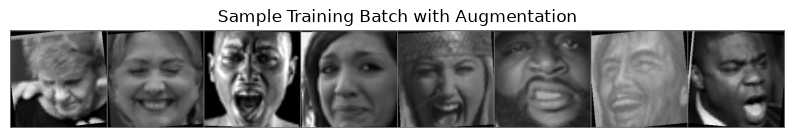
\includegraphics[width=0.9\textwidth]{images/sample_batch.png}
    \caption{نمونه‌ای از داده‌های آموزش پس از تغییر ابعاد به $224 \times 224$، سه‌کاناله شدن و اعمال افزونگی داده. نرمال‌سازی برای نمایش معکوس شده است.}
    \label{fig:sample_batch}
\end{figure}

همان‌طور که در شکل \ref{fig:sample_batch} مشخص است، ماهیت احساسات در تصاویر \lr{(Semantic Meaning)} حفظ شده و تغییرات هندسی اعمال‌شده در بازه‌ی منطقی و واقع‌گرایانه قرار دارند.